\documentclass[conference]{IEEEtran}
\IEEEoverridecommandlockouts
% The preceding line is only needed to identify funding in the first footnote. If that is unneeded, please comment it out.
\usepackage[T1]{fontenc}
\usepackage{algorithm} 
\usepackage{tgbonum}
\usepackage{algpseudocode}
\usepackage{hyperref}
\usepackage{enumerate}
\usepackage{fontspec}
\usepackage{adjustbox}
\usepackage{cite}
\usepackage{amsmath,amssymb,amsfonts}
\usepackage{algorithmicx}
\usepackage{graphicx}
\usepackage{textcomp}
\usepackage{xcolor}
\algnewcommand{\Inputs}[1]{%
  \State \textbf{Inputs:}
  \Statex \hspace*{\algorithmicindent}\parbox[t]{.8\linewidth}{\raggedright #1}
}
\algnewcommand{\Initialize}[1]{%
  \State \textbf{Initialize:}
  \Statex \hspace*{\algorithmicindent}\parbox[t]{.8\linewidth}{\raggedright #1}
}

\def\BibTeX{{\rm B\kern-.05em{\sc i\kern-.025em b}\kern-.08em
    T\kern-.1667em\lower.7ex\hbox{E}\kern-.125emX}}
\title{%
  Design and Analysis of Algorithms \\
  \large Assignment 3\\
  Group 16
    \author{\IEEEauthorblockN{Gaurav N\IEEEauthorrefmark{1},
Vinit W\IEEEauthorrefmark{2}and Prince\IEEEauthorrefmark{3}}
\IEEEauthorblockA{Department of Information Technology,
Indian Institute of Information Technology\\
Allahabad\\
ID: \IEEEauthorrefmark{1}IIT2019231,
\IEEEauthorrefmark{2}IIT2019232,
\IEEEauthorrefmark{3}IIT2019233}}}


\begin{document}
{\fontfamily{qag}\selectfont


\maketitle
\thispagestyle{plain}
\pagestyle{plain}

\begin{abstract}
For a given large binary string, the project aims at calculating the length of substring which is having maximum difference of number of 0s and number of 1s.\\
\end{abstract}



\section{Introduction}
A string that consists of only 1's ans 0's is said to be a binary string.\\

In our project, we tested  various algorithms on different sample test cases for time complexity and space complexity. In our report, we tend to focus on establishing a rule or a relationship between the time and input data.\\

We have analysed three different approaches -
\begin{enumerate}[(i)]
    \item Brute force
    \item Recursive 2D DP
    \item Iterative 1D DP\\
\end{enumerate}



This report further contains -

II. \nameref{algodesign}

III. \nameref{algoimple}

IV. \nameref{algoanalysis}

V. \nameref{expstudy}

VI. \nameref{conclusion}\\

\section{Algorithm Design}
\label{algodesign}

\begin{enumerate}[A)]
  
  \item Brute force -
  \begin{enumerate}
    \item Approach:
    
       In brute force implementation, for every possible sub array of every possible size, we calculate difference of number of 0's and number of 1's. This can be done using combination of 3 nested loops. We keep track of the maximum value of difference and corresponding sub array size till that instant and print its value in the end.
    \item Algorithm:
    \begin{enumerate}
    \item The outermost loop keeps track of current size of the sub array.
    \item The middle loop will keep track of current starting index of the sub array.
    \item The innermost loop will traverse the current sub array and count the number of 0's and number of 1's for it.
\item For every sub array, we find the difference of number of 0's and number of 1's. If this difference exceeds maximum value of difference till that instant, we assign current difference's value to maximum difference and update size accordingly.
\item Finally, we print the size of the sub array corresponding to the maximum value of difference.\\
    \end{enumerate}
    \end{enumerate}
    
    \item Recursive 2D DP - 
    Dynamic programming involves dividing a problem into similar sub-problems, and reusing the already calculated results for sub problems.

    \begin{enumerate}
    \item Approach:
    
    In this approach, we will convert given binary string into integer array such that if \textit{$string[i]=‘0’$} then \textit{$arr\textsubscript{i}=-1$} and if \textit{$string[i]=‘1’$} then \textit{$arr\textsubscript{i}=1$}. Now, for each index we need to make decision whether to take it or skip it. So, we declare a 2D array to memorize result for that index.
    \item Algorithm:
    \begin{enumerate}
    \item The idea is to recursively find size of sub array corresponding to indices until base case (i.e. end of the binary string is reached).
\item Create a function that checks if the given binary string consists of all 1's. If it consists of all 1's, the answer will be 0.
\item Create a recursive function to calculate maximum difference of number of 0's and number of 1's corresponding to each index in the given binary string.
\item The base case of recursion is when end of the given binary string is reached.
\item Print the answer.\\
\end{enumerate}
    \end{enumerate}
    
    \item Iterative 1D DP - 
    Given an array, Kadane’s algorithm is able to find the maximum sum and size of a contiguous sub array in an array with a run time of O(n). Kadane's algorithm uses the concept of dynamic programming.
    \begin{enumerate}
    \item Approach:
    
     In this approach, we convert all 0's in the binary string into 1's and all 1's into -1's. Now, all we have to do is to find out the size of sub array with maximum Using Kadane’s Algorithm.
    \item Algorithm:
    \begin{enumerate}
    \item In this implementation, we traverse the binary string from left to right.
    \item We maintain four variables. They will signify  values of current sum, maximum sum  and current size, maximum size.
    \item If the \textit{$i^t$}\textit{$^h$} character of the binary string is \textit{$0$} then we will add \textit{$1$} to the current sum else we will decrement current sum by \textit{$1$}.
    \item At any instant, if current sum becomes less than 0, we set current sum and current size to zero.
    \item At any instant, if current sum becomes greater than maximum sum, we set maximum sum to current sum and maximum size to current size.
    \item Print maximum size.\\
\end{enumerate}
    \end{enumerate}
    
  \end{enumerate}

\section{Algorithm Implementation}
\label{algoimple}


% \begin{algorithm}
%     \caption{Brute Force}\label{your_label1}
%     \begin{algorithmic}
%     \Inputs{$N$, $string$ $str$}
%     \Procedure{findSize}{$N$, $string$ $str$}
%         \Initialize{\strut $size$ = 0, \strut $count0s$ = 0, \strut $count1s$ = 0, \strut $length_\mathrm{max}$ = 0, \strut $diff_\mathrm{max}$ = 0}
%         \If{$length=1$}
%                 \State \Return $arr$
%         \EndIf
%         \Initialize{\strut $midPoint=length/2$}
%         \Initialize{\strut 
%         $firstHalf,inversions1 = \Call {countInversions}{\mathrm{arr}_\mathrm{first half}}$}
%         \Initialize{\strut 
%         $secondHalf,inversions2 = \Call {countInversions}{\mathrm{arr}_\mathrm{second half}}$}
%         \Initialize{\strut $sortedArray = [...]$, $i=0$, $j=0$ and $inversions=0$}
%         \While{($i< \mathrm{length}_\mathrm{first half}$ and $j< \mathrm{length}_\mathrm{second half})$ }
%           \If{$\mathrm{arr}_\mathrm{first half}[i]$>$\mathrm{arr}_\mathrm{second half}[j]$}
%                 \State {$append$ $\mathrm{arr}_\mathrm{second half}[j]$ $to$ $sortedArray$
%                 \State $inversions=inversions+(midPoint-i)$}
%             \Else
%                 \State $append$ $\mathrm{arr}_\mathrm{first half}[i]$ $to$ $sortedArray$
%             \EndIf
%         \EndWhile
%         \State $append$ remaining $\mathrm{arr}_\mathrm{first half}$ $to$ $sortedArray$
%         \State $append$ remaining $\mathrm{arr}_\mathrm{second half}$ $to$ $sortedArray$
%         \State $totalInversions = inversions1 + inversions2 + inversions$
%         \State \Return {$sortedArray, totalInversions$}
%     \EndProcedure
% \end{algorithmic}
% \end{algorithm}

% \begin{algorithm}
%     \caption{Recursive 2D DP}\label{your_label2}
%     \begin{algorithmic}
%     \Inputs{$N$, $arr$ = [$a_i$ for $0 <= i <|arr|$]}
%     \Procedure{countInversions}{$arr$}
%         \Initialize{\strut $length$ = length of arr}
%         \If{$length=1$}
%                 \State \Return $arr$
%         \EndIf
%         \Initialize{\strut $midPoint=length/2$}
%         \Initialize{\strut 
%         $firstHalf,inversions1 = \Call {countInversions}{\mathrm{arr}_\mathrm{first half}}$}
%         \Initialize{\strut 
%         $secondHalf,inversions2 = \Call {countInversions}{\mathrm{arr}_\mathrm{second half}}$}
%         \Initialize{\strut $sortedArray = [...]$, $i=0$, $j=0$ and $inversions=0$}
%         \While{($i< \mathrm{length}_\mathrm{first half}$ and $j< \mathrm{length}_\mathrm{second half})$ }
%           \If{$\mathrm{arr}_\mathrm{first half}[i]$>$\mathrm{arr}_\mathrm{second half}[j]$}
%                 \State {$append$ $\mathrm{arr}_\mathrm{second half}[j]$ $to$ $sortedArray$
%                 \State $inversions=inversions+(midPoint-i)$}
%             \Else
%                 \State $append$ $\mathrm{arr}_\mathrm{first half}[i]$ $to$ $sortedArray$
%             \EndIf
%         \EndWhile
%         \State $append$ remaining $\mathrm{arr}_\mathrm{first half}$ $to$ $sortedArray$
%         \State $append$ remaining $\mathrm{arr}_\mathrm{second half}$ $to$ $sortedArray$
%         \State $totalInversions = inversions1 + inversions2 + inversions$
%         \State \Return {$sortedArray, totalInversions$}
%     \EndProcedure
% \end{algorithmic}
% \end{algorithm}


\begin{algorithm}
    \caption{Iterative 1D DP}\label{your_label3}
    \begin{algorithmic}
    \Inputs{$N$, $string$ $str$}
    \Procedure{findMaxLength}{$N$, $string$ $str$}
        \Initialize{\strut $sum_\mathrm{max}$ = 0, \strut $sum_\mathrm{current}$ = 0,\strut $size_\mathrm{max}$ = 0, \strut $size_\mathrm{current}$ = 0, \strut $i$ = 0}
        \For{\textit{i = 0; i < n; i++}}
            \If{$str_\mathrm{i}==0$}
                \State $sum_\mathrm{current}=sum_\mathrm{current}+1$
            \Else
                \State $sum_\mathrm{current}=sum_\mathrm{current}-1$
            \EndIf
            \State $size_\mathrm{current}=size_\mathrm{current}+1$
            \If{$sum_\mathrm{current}<0$}
                \State $sum_\mathrm{current}=0$
                \State $size_\mathrm{current}=0$
            \EndIf
            \If{$sum_\mathrm{current}>sum_\mathrm{max}$}
                \State $sum_\mathrm{max}=sum_\mathrm{current}$
                \State $size_\mathrm{max}=size_\mathrm{current}$
            \EndIf
        \EndFor
        \State \Return {$size_\mathrm{max}$}
    \EndProcedure
\end{algorithmic}
\end{algorithm}

\section{Algorithm Analysis}
\label{algoanalysis}

\begin{enumerate}[A)]
 
 \item
Brute force:

In case of brute force algorithm, three nested loops are needed to for calculation of difference of number of 0's and number of 1's for all possible sub arrays, so the overall time complexity is O($n^3$) while no extra space is required resulting into O(1) space complexity.

\centerline{Time complexity:O($n^3$)}
\centerline{Space complexity:O(1)}.

\item 
Recursive 2D DP:

In case of recursive implementation, the concept of 2D dynamic programming is used. The height of the recursive tree is same as the length of the given binary string, so the time complexity is O(n). The memorization for the DP will also be proportional to the length of the given binary string, resulting in O(n) space complexity.

\centerline{Time complexity:O(n)}
\centerline{Space complexity:O(n)}.
\item 
Iterative 1D DP:

In case of iterative implementation, the concept of 1D dynamic programming is used. One full array traversal is needed, so the time complexity is O(n). In this implementation, we don't need to tabulate all the sub results, but only the recently derived ones. This results in O(1) space complexity.

\centerline{Time complexity:O(n)}
\centerline{Space complexity:O(1)}.
\end{enumerate}


\section{Experimental Study}
\label{expstudy}
\begin{figure}[ht]
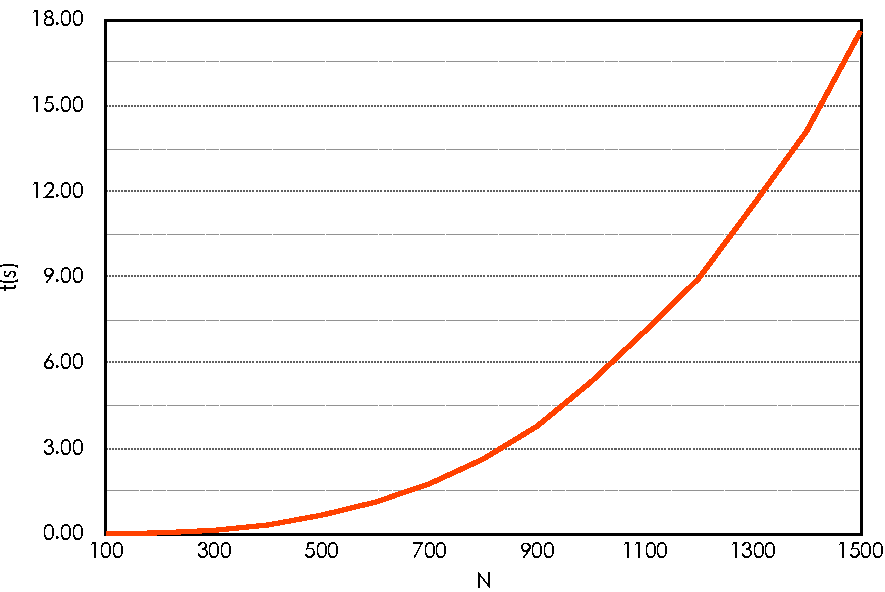
\includegraphics[scale=0.6]{Brute Force.pdf}
\caption{N vs t for Brute force algorithm}
\end{figure}


\begin{figure}[ht]
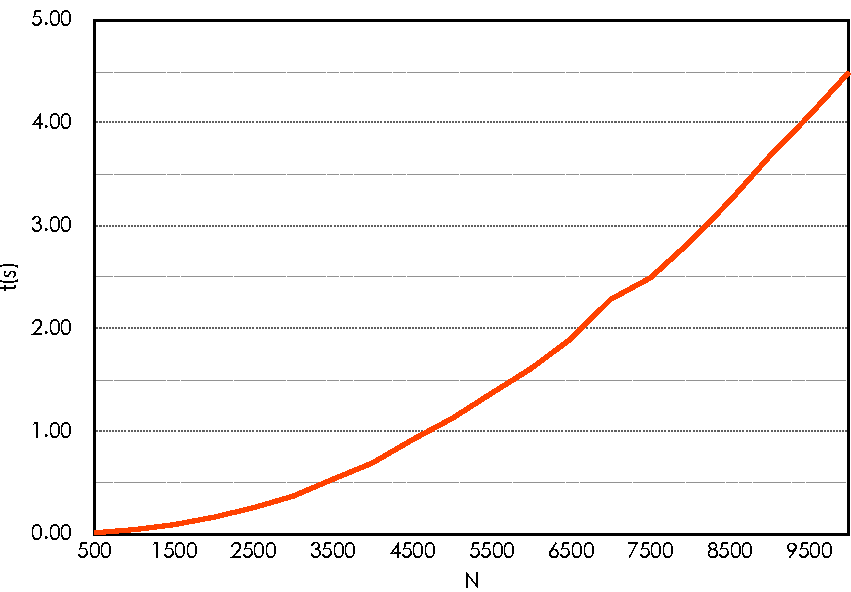
\includegraphics[scale=0.6]{Recursive 2D DP.pdf}
\caption{N vs t for Recursive 2D DP algorithm}
\end{figure}


\begin{figure}[ht]
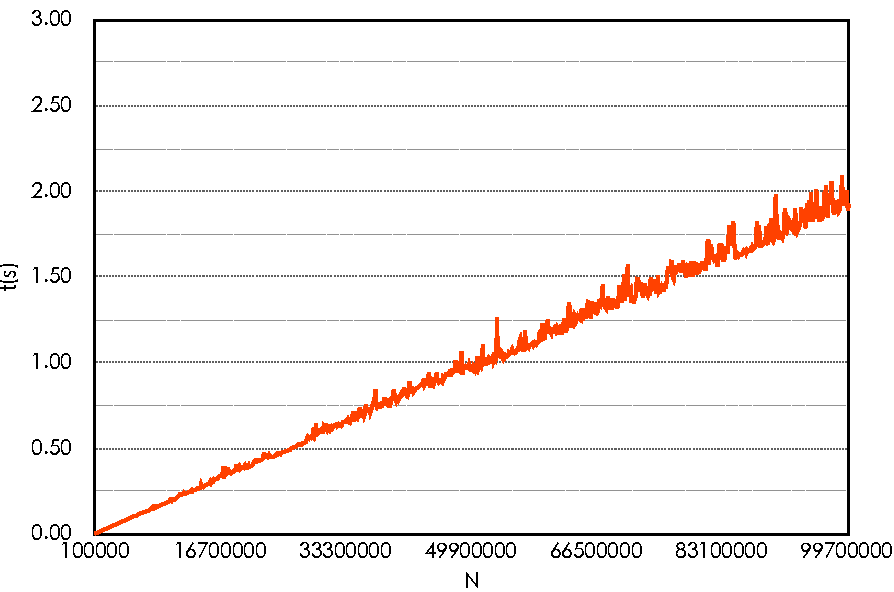
\includegraphics[scale=0.6]{Iterative 1D DP.pdf}
\caption{N vs t for Iterative 1D DP algorithm}
\end{figure}

Fig. 1. The graph for the first algorithm shows the non-linear behaviour as n increases, this behaviour is in fact of
$n^3$.\\

Fig. 2. The graph for the second algorithm shows almost linear behaviour as n increases, this behaviour is in fact of
$n$.\\

Fig. 3. The graph for the second algorithm shows the linear behaviour as n increases, this behaviour is in fact of
$n$.\\



\section{Conclusion}
\label{conclusion}
From the mutual graphs of all three algorithms derived from experimental studies, we can conclude that the average running time of naive brute force implementation is worst of all three. The recursive 2D DP implementation takes significantly less time than plane brute force algorithm. By comparing the graphs of recursive and iterative algorithms, we can conclude that the iterative 1D DP algorithm is the fastest one.

One thing to note, as we have shown before in the algorithm analysis, the time complexity of recursive and iterative implementation both is the same i.e O(n). But after experimental analysis, we can see that the iterative algorithm performs significantly better than recursive one. This difference can be mapped to the fact that memorization can be slower than tabulation because of large number of recursive calls. Also, in the recursive implementation, we have to initialize memorization container of length n, while space needed in tabulation approach is constant.

One other disadvantage of recursive implementation is that for large binary strings, the recursion tree will be very deep, which  will result into system running out of stack space and thereafter the program will crash.

\begin{thebibliography}{00}
\bibitem{b1} https://www.geeksforgeeks.org/maximum-difference-zeros-ones-binary-string/
\bibitem{b2} https://www.geeksforgeeks.org/maximum-difference-zeros-ones-binary-string-set-2-time/
\end{thebibliography}
}
\end{document}
